\section{Spin responses from neutron data}\label{sec:14.4}

The full magnon spectrum of YIG, all twenty branches up to about \SI{110}{meV}, has been measured by inelastic neutron scattering with neutrons of \SI{120}{meV}~\cite{princep2017full,berlin2025determining}. Such a neutron carries \SI{15.0}{keV} of momentum, the largest momentum of a dark-matter particle of \SI{5.7}{MeV}, and its spin couples to the spin density $\vect{s}_e(\vect{q})$ (\cref{app:C.19}). The measured cross-section can therefore replace the model response of \cref{sec:14.1}, with every magnon branch, every multi-magnon process and the magnetic form factor already included, as Berlin, Millar, Trickle and Zhou did for YIG~\cite{berlin2025determining}. A neutron, however, couples only to the part of the spin density perpendicular to the momentum transfer, and how much of the dark-matter response that part fixes depends on the coupling and on how much model input is added for the magnet.

\subsection{Conversion of neutron spectra}

Neutron spectra are reported per formula unit of the crystal. With $N_{\mathrm{fu}}$ formula units in a cell of volume $\Omega$, the measured magnetic structure factor $S^{\mathrm{neu}}(\vect{q},\omega)$ is defined by $\dd^2\sigma/\dd\Omega\,\dd E' = (p'_n/p_n)\,S^{\mathrm{neu}}$ for one formula unit, with $\dd\Omega$ here the solid angle of the outgoing neutron. Dividing \cref{eq:C.19-cross} by the number of formula units in the sample, $\Vol N_{\mathrm{fu}}/\Omega$, and solving for the response,
\begin{equation}
  \Tr\bigl[P_T\,S(\vect{q},\omega)\bigr] = \sum_{a,b}(P_T)_{ab}\,S_{ab}(\vect{q},\omega) = \frac{2\pi N_{\mathrm{fu}}}{(\gamma_nr_{\mathrm{cl}})^2\,\Omega}\,S^{\mathrm{neu}}(\vect{q},\omega) ,
  \label{eq:14.4-PT}
\end{equation}
with $(P_T)_{ab} = \delta_{ab} - \hat q_a\hat q_b$ and $(\gamma_nr_{\mathrm{cl}})^2 = \SI{0.2906}{b}$. This is the relation of Berlin et al.~\cite[Eq.~(26)]{berlin2025determining}. The thermal vibration of the ions enters through the Debye--Waller factor, which the dark matter sees in the same way, so it stays inside $S_{ab}$ (\cref{app:C.19}).

Two corrections, for temperature and for the orbital moment, turn \cref{eq:14.4-PT} into the response that a detector needs. The spectrum is measured at a temperature $T_{\mathrm{d}}$, below \SI{10}{K} for the YIG data~\cite[App.~B\,2]{berlin2025determining}, while a detector runs at millikelvin. By the fluctuation--dissipation theorem \cref{eq:4.2-fdt}, $(1 - \ee^{-\beta\omega})S_{ab}$ is the dissipative response, and for free magnons this response does not depend on temperature, as for the thermal oscillator of \cref{sec:4.2}. Hence
\begin{equation*}
  S_{ab}(\vect{q},\omega;T \to 0) = \bigl(1 - \ee^{-\omega/T_{\mathrm{d}}}\bigr)\,S_{ab}(\vect{q},\omega;T_{\mathrm{d}}) , \qquad \omega > 0 ,
\end{equation*}
which removes the thermal population of the measured spectrum. The residual is set by the magnon interactions, which make the response follow the thermal reduction of the ordered moment; it is small for $T_{\mathrm{d}}$ well below the ordering temperature.

The second correction is the orbital moment. A neutron couples to the magnetization, spin and orbital, while spin-coupled dark matter couples to the spin alone. For a quenched $3d$ ion of spin $\vect{S}$, \cref{sec:14.3} showed that spin--orbit coupling induces an orbital moment $\vect{L} = (g_{\mathrm{ion}} - 2)\vect{S}$ at first order, with $g_{\mathrm{ion}}$ the spectroscopic $g$ factor of the ion (\cref{sec:14.3-lande}), taken isotropic here, while the spin itself changes only at second order, $\lambda_S = 1 - O(\xi_{\mathrm{ion}}^2/\Delta_{\mathrm{CF}}^2)$. In the dipole approximation of \cref{app:C.19} the spin part of the moment carries the radial integral $\langle j_0\rangle$ and the orbital part $\langle j_0\rangle + \langle j_2\rangle$. The moment $2\vect{S}\langle j_0\rangle + \vect{L}(\langle j_0\rangle + \langle j_2\rangle)$ is then $g_{\mathrm{ion}}\vect{S}\,F^{\mathrm{mag}}_g(q)$, and the neutron couples to
\begin{equation*}
  \vect{s}_e(\vect{q}) \to \frac{g_{\mathrm{ion}}}{2}\,F^{\mathrm{mag}}_g(q)\sum_j\ee^{\ii\vect{q}\cdot\vect{R}_j}\vect{S}_j, \qquad F^{\mathrm{mag}}_g(q) = \langle j_0(q)\rangle + \Bigl(1 - \frac2g\Bigr)\langle j_2(q)\rangle ,
\end{equation*}
while the dark matter couples to $\lambda_S\langle j_0(q)\rangle\sum_j\ee^{\ii\vect{q}\cdot\vect{R}_j}\vect{S}_j$. The two operators differ by a number at each $q$, so their responses differ by its square:
\begin{keyresult}[Data-driven spin response]
\begin{equation}
  \Tr\bigl[P_T\,S(\vect{q},\omega)\bigr] = C_{\mathrm{sn}}(q)\,\frac{2\pi N_{\mathrm{fu}}}{(\gamma_nr_{\mathrm{cl}})^2\,\Omega}\,S^{\mathrm{neu}}(\vect{q},\omega), \qquad
  C_{\mathrm{sn}}(q) = \biggl[\frac{\lambda_S\,\langle j_0(q)\rangle}{(g_{\mathrm{ion}}/2)\,F^{\mathrm{mag}}_g(q)}\biggr]^2 ,
  \label{eq:14.4-data}
\end{equation}
for one species of quenched magnetic ion, with $S_{ab}$ the response of the electron spin density and $S^{\mathrm{neu}}$ measured per formula unit, its thermal population removed. At $q \to 0$, $C_{\mathrm{sn}} = [\lambda_S/(g_{\mathrm{ion}}/2)]^2$.
\end{keyresult}
\noindent For an anisotropic $g_{\mathrm{ion}}$ tensor, $g_{\mathrm{ion}}/2$ becomes the matrix $g_{\mathrm{ion},ab}/2$ acting on both indices of $S_{ab}$. For a $J$ multiplet, $g_{\mathrm{ion}}$ is replaced by $g_J$, $\lambda_S$ by $g_J - 1$ (\cref{eq:14.3-gJ}) and $F^{\mathrm{mag}}_g$ by the dipole form factor \cref{eq:C.19-dipole}; at $q \to 0$, $C_{\mathrm{sn}}$ is the square of the last column of \cref{tab:14-lande}. It is 1 for Gd$^{3+}$, $\frac19$ for Er$^{3+}$ and 25 for Sm$^{3+}$, whose spin points against its moment.

For Ni$^{2+}$ in NiO, $g_{\mathrm{ion}} = 2.18 \simeq 2.2$~\cite{kritzell2024terahertz}. With $\lambda_S = 1$,
\begin{equation*}
  C_{\mathrm{sn}}(0) = \Bigl(\frac{2}{2.2}\Bigr)^2 = 0.83 :
\end{equation*}
the spin response of NiO is \SI{17}{\percent} below what the neutron cross-section suggests if read as pure spin. Setting $\lambda_S = g_{\mathrm{ion}} - 1$ instead, the rule that holds only for $J$ multiplets, would give $(1.2/1.1)^2 = 1.19$ and an error of the opposite sign. The $q$ dependence enters through $\langle j_2\rangle$, which vanishes at $q = 0$ and grows with $q$. With the tabulated radial integrals of Ni$^{2+}$~\cite[Sect.~4.4.5]{anderson2006neutron}, the same fit form as for $\langle j_0\rangle$ in \cref{sec:14.1} multiplied by $s^2$ with coefficients $(1.708, 11.016, 1.2147, 4.103, 0.315, 1.533, 0.0018)$, the ratio $\langle j_2\rangle/\langle j_0\rangle$ is 0.035 at $|\vect{Q}_{\mathrm{AF}}| = \SI{2.6}{keV}$ and 0.15 at \SI{5.3}{keV}. $C_{\mathrm{sn}}(q)/C_{\mathrm{sn}}(0)$ is then 0.994 and 0.973, and it stays within \SI{10}{\percent} of one up to \SI{10}{keV}. The value of $g_{\mathrm{ion}}$ is the larger uncertainty. Magnetic x-ray diffraction on NiO, which separates the spin and orbital moments, finds $L/S = 0.34$~\cite{fernandez1998observation}, and DFT~$+\,U$ with spin--orbit coupling gives 0.36~\cite{kwon2000unquenched}. Read in the quenched picture as $g_{\mathrm{ion}} = 2 + L/S = 2.34$, this lowers $C_{\mathrm{sn}}(0)$ to 0.73, \SI{12}{\percent} below the value at $g_{\mathrm{ion}} = 2.2$. The orbital moment of Ni$^{2+}$ is thus an uncertainty of about \SI{10}{\percent} on the normalization of the data-driven rate. The $g_{\mathrm{ion}}$ tensor and the orbital moments are computed in DFT~$+\,U$ with spin--orbit coupling (\cref{app:E.20-magnet}), and the radial integrals from Dirac--Fock or Wannier-projected shells.

\Cref{lim:14.4a} shows how far the spin-only reading of the data holds as the orbital admixture grows.
\begin{limitbox}[Data-driven spin response][lim:14.4a]
$\Tr[P_TS(\vect{q},\omega)] = 2\pi N_{\mathrm{fu}}S^{\mathrm{neu}}(\vect{q},\omega)/[(\gamma_nr_{\mathrm{cl}})^2\Omega]$, for a neutron coupled to the electron spin alone~\cite[Eqs.~(8), (11), (26)]{berlin2025determining}.
\par\smallskip
{\centering
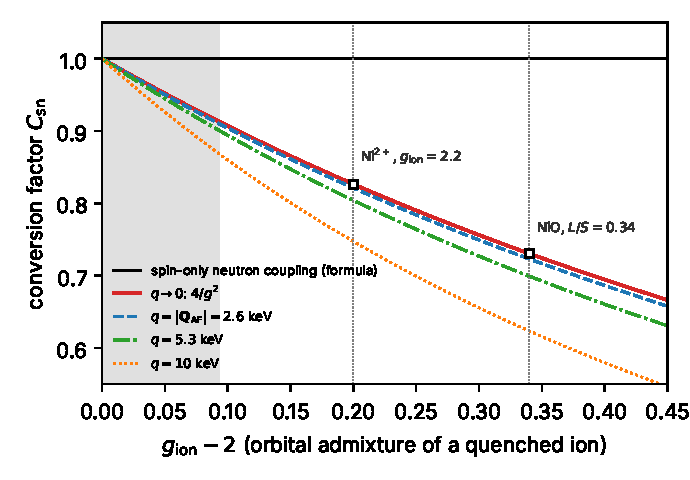
\includegraphics[width=0.78\linewidth]{figures/ch14/limit14_4a.pdf}
\captionof{figure}{Ratio of the spin response to the response inferred from neutron data by the spin-only formula, $C_{\mathrm{sn}}(q)$ of \cref{eq:14.4-data}, against the shift $g_{\mathrm{ion}} - 2$ of the spectroscopic $g_{\mathrm{ion}}$ factor of a quenched ion, with $\lambda_S = 1$ and the dipole form factor $\langle j_0\rangle + (1 - 2/g_{\mathrm{ion}})\langle j_2\rangle$. Black: the formula, ratio 1. Red: $q \to 0$, $4/g^2$. Dashed, dash-dotted and dotted: $q = \SI{2.6}{keV}$ (the ordering wavevector of NiO), \SI{5.3}{keV} (largest momentum transfer at $\mchi = \SI{1}{MeV}$) and \SI{10}{keV}, with the radial integrals of Ni$^{2+}$. Squares: $g_{\mathrm{ion}} = 2.2$ (octahedral Ni$^{2+}$) and $g_{\mathrm{ion}} = 2.34$ (NiO with $L/S = 0.34$ from magnetic x-ray diffraction). Gray: $g_{\mathrm{ion}} - 2 \le 0.094$, where the formula holds within \SI{10}{\percent} for $q \le \SI{5.3}{keV}$.}\label{fig:14-limit-neutron}
\par}
\smallskip
Outside the gray band the orbital moment shifts the neutron response from the spin response at first order in $g_{\mathrm{ion}} - 2$, and at large $q$ the orbital form factor $\langle j_2\rangle$ adds to the shift.
\end{limitbox}

How much of the dark-matter kinematic region the data reach depends on the instrument. In the YIG spectrum of Berlin et al.\ the data below \SI{5}{meV} are dominated by elastic scattering and are discarded, and the crystal was rotated about one axis only, so at large $q$ only a narrow band of directions $\hat{\vect{q}}$ is covered~\cite[Sect.~III\,B and App.~D]{berlin2025determining}. Averaging $S^{\mathrm{neu}}$ over the covered directions at fixed $|\vect{q}|$ and $\omega$ is justified well outside the first zone, since a small change in the direction of $\vect{q}$ moves its reduced part across the whole zone. Below a mass of \SI{134}{keV}, where $2\mchi v_{\mathrm{max}}$ reaches the radius $\sqrt2\pi/a = \SI{708}{eV}$ of the largest sphere inside the zone, every momentum transfer lies inside the first zone, where there are few data, and the data-driven reach falls rapidly below about \SI{200}{keV}. Near \SI{1}{MeV} the data-driven rate agrees closely with the Heisenberg-model rate fitted to the same spectrum~\cite[Fig.~3]{berlin2025determining}. At larger masses the data contain the form factor of Fe$^{3+}$, which the model omits and which suppresses the rate by an order of magnitude for $q \gtrsim \SI{10}{keV}$. They also contain phonons, excited by the nuclear scattering of the neutron with a relative weight that grows as $q^2/(M\omega)$, about $(q/\SI{30}{keV})^2$ for nuclei of \SI{50}{GeV} and $\omega \sim \SI{20}{meV}$~\cite[App.~C]{berlin2025determining}. Spin-flip scattering with the polarization along $\hat{\vect{q}}$ contains all the magnetic scattering and no coherent nuclear scattering (\cref{app:C.19}), and it removes the phonons without a model, up to the two thirds of the nuclear-spin-incoherent scattering that it keeps, which is small for Y, Fe and O. A modelled phonon part subtracted from unpolarized data must leave a response that is still positive semidefinite (\cref{eq:4.2-positivity}).

\subsection{Transverse projection of the neutron cross-section}

Which couplings \cref{eq:14.4-PT} calibrates depends on the dark-matter tensor $\mathfrak{D}_{ab}$ of \cref{eq:8.1-D} for the spin row. For the operators of \cref{tab:8-operators} with dark matter of spin $\frac12$ there are three structures. The contact interaction $\mathcal{O}_4$ gives $\mathfrak{D}_{ab} = |c_4^{(e)}|^2\delta_{ab}/4$. The pseudoscalar couplings give $\hat q_a\hat q_b$: $\mathcal{O}_{10}$ gives $|c_{10}^{(e)}|^2q_aq_b/m_e^2$ and $\mathcal{O}_6$ gives $|c_6^{(e)}|^2q^2q_aq_b/4m_e^4$. Operator $\mathcal{O}_9 = \ii\vect{S}_\chi\cdot(\vect{S}_e\times\vect{q}/m_e)$, and the spin--spin part $(\vect{S}_\chi\times\vect{q})\cdot(\vect{S}_e\times\vect{q})$ of magnetic-dipole and anapole dark matter, give the transverse projector: for $\mathcal{O}_9$, $\Tr_\chi[(\vect{q}\times\vect{S}_\chi)_a(\vect{q}\times\vect{S}_\chi)_b]/2 = q^2(P_T)_{ab}/4$, so $\mathfrak{D}_{ab} = |c_9^{(e)}|^2q^2(P_T)_{ab}/4m_e^2$. Since $\delta_{ab} = (P_T)_{ab} + \hat q_a\hat q_b$, the three contractions are
\begin{equation}
  \sum_{a,b}\delta_{ab}S_{ab} = \Tr\bigl[P_TS\bigr] + \hat{\vect{q}}\cdot S\cdot\hat{\vect{q}}, \qquad \sum_{a,b}(P_T)_{ab}S_{ab} = \Tr\bigl[P_TS\bigr], \qquad \sum_{a,b}\hat q_a\hat q_bS_{ab} = \hat{\vect{q}}\cdot S\cdot\hat{\vect{q}} .
  \label{eq:14.4-split}
\end{equation}
The neutron data fix the transverse couplings completely: the rates of $\mathcal{O}_9$, magnetic-dipole and anapole dark matter follow from \cref{eq:8.2-spectrum} with $S^{\mathrm{neu}}$ and nothing else. For $\mathcal{O}_4$, however, the transverse part alone is only a lower bound on the rate of the contact interaction: the longitudinal element $\hat{\vect{q}}\cdot S\cdot\hat{\vect{q}}$ is a diagonal element of a positive semidefinite matrix and cannot be negative. For $\mathcal{O}_6$ and $\mathcal{O}_{10}$ the data at one $\vect{q}$ leave the rate unconstrained. Tensors built from the dark-matter velocity, as for $\mathcal{O}_7$ and $\mathcal{O}_{12}$--$\mathcal{O}_{15}$, also need the mixed elements between the direction of $\vect{q}$ and the two directions perpendicular to it.

Absorption needs exactly the missing element. The spin row of an axion-like particle is proportional to its momentum, and the absorption rate \cref{eq:14.3-abs} contracts $S_{ab}$ with $p_{\phi,a}p_{\phi,b}$: it is $p_\phi^2\,\hat{\vect{p}}_\phi\cdot S\cdot\hat{\vect{p}}_\phi$, a longitudinal element~\cite[Eqs.~(15), (17)]{berlin2025determining}. Its momentum, $p_\phi \sim 10^{-3}m_\phi$, is also far below any momentum transfer a neutron spectrometer resolves. At $q \to 0$ the full tensor is fixed instead by the magnetic permeability measured in resonance or terahertz experiments~\cite[footnote~3]{berlin2025determining}, and in the model of \cref{sec:14.3} by the Larmor and Kittel lines.

That the longitudinal element is missing at each $q$, whatever the beam, follows from the form of the amplitude. \Cref{fig:14-neutron} shows the geometry.
\begin{keyresult}[Neutron scattering and the longitudinal spin response]
At a given $\vect{q}$, magnetic neutron scattering measures only the block of $S_{ab}(\vect{q},\omega)$ transverse to $\hat{\vect{q}}$: unpolarized beams its trace $\Tr[P_TS]$, polarization analysis its elements. Without a model of the magnet (of the spin density within the cell, or the spin-isotropy hypothesis of \cref{sec:14.4-iso}), the longitudinal element $\hat{\vect{q}}\cdot S\cdot\hat{\vect{q}}$ and the mixed elements between $\hat{\vect{q}}$ and the transverse plane are measured by no neutron experiment, polarized or not, and no symmetry of the crystal relates them to the transverse block at the same $\vect{q}$. Within the localized-moment model of \cref{eq:14.4-data}, transverse data at several wavevectors $\vect{q} + \vect{G}$ determine the full tensor.
\end{keyresult}
\noindent The first part is the perpendicular-projection rule of magnetic neutron scattering (\cref{app:C.19}). Every amplitude in \cref{eq:C.19-amplitude,eq:C.19-polar} contains $\vect{s}_e$ only through $\vect{s}_\perp = P_T\vect{s}_e$, because a spin density modulated along $\vect{q}$ produces no magnetic field at that wavevector (\cref{eq:C.19-field}). In the frame of \cref{app:C.19}, with $x$ along $\hat{\vect{q}}$, polarization analysis separates $S_{yy}$, $S_{zz}$ and the chiral part of $S_{yz}$, and full polarimetry reaches its symmetric part as well~\cite{blume1963polarization}. That is at most four of the nine real numbers of the Hermitian matrix $S_{ab}$.

For the second part, let $\mathsf{h}$ be an element of the magnetic point group, acting as a rotation matrix $\mathsf{R}$ on positions and on the axial spin. It maps the response at $\vect{q}$ onto the response at $\mathsf{R}\vect{q}$, $S(\mathsf{R}\vect{q}) = \mathsf{R}\,S(\vect{q})\,\mathsf{R}^{\mathrm{T}}$, possibly transposed if $\mathsf{h}$ contains time reversal; the transpose does not change the symmetric contractions. Since also $P_T(\mathsf{R}\hat{\vect{q}}) = \mathsf{R}\,P_T(\hat{\vect{q}})\,\mathsf{R}^{\mathrm{T}}$,
\begin{equation*}
  \Tr\bigl[P_T(\mathsf{R}\hat{\vect{q}})\,S(\mathsf{R}\vect{q})\bigr] = \Tr\bigl[\mathsf{R}P_T(\hat{\vect{q}})\mathsf{R}^{\mathrm{T}}\mathsf{R}S(\vect{q})\mathsf{R}^{\mathrm{T}}\bigr] = \Tr\bigl[P_T(\hat{\vect{q}})\,S(\vect{q})\bigr] ,
\end{equation*}
and a measurement at a symmetry-equivalent wavevector repeats the same equation. The elements that leave $\hat{\vect{q}}$ fixed map the direction of $\vect{q}$ onto itself and the transverse plane onto itself, so they constrain the transverse block and the longitudinal element separately and never relate one to the other. A wavevector $\vect{q} + \vect{G}$ that points elsewhere belongs to a different operator, $\vect{s}_e(\vect{q} + \vect{G})$, which the exact response does not tie to $\vect{s}_e(\vect{q})$.

The localized-moment form that \cref{eq:14.4-data} already uses supplies that tie. For one magnetic ion per primitive cell, as for NiO in its chemical cell, $\vect{s}_e(\vect{k} + \vect{G}) = F^{\mathrm{mag}}(|\vect{k} + \vect{G}|)\sum_j\ee^{\ii(\vect{k}+\vect{G})\cdot\vect{R}_j}\vect{S}_j$ with $\ee^{\ii\vect{G}\cdot\vect{R}_j} = 1$, so that
\begin{equation}
  S_{ab}(\vect{k} + \vect{G},\omega) = |F^{\mathrm{mag}}(|\vect{k} + \vect{G}|)|^2\,\ee^{-2W(\vect{k}+\vect{G})}\,S^{\mathrm{lat}}_{ab}(\vect{k},\omega) ,
  \label{eq:14.4-Glat}
\end{equation}
for every reciprocal vector $\vect{G}$, with $S^{\mathrm{lat}}$ the response of the lattice spins and the Debye--Waller factor $\ee^{-2W}$ taken at $\vect{k} + \vect{G}$, beside the form factor. Each $\vect{G}$ gives the transverse trace $\Tr S^{\mathrm{lat}} - \hat{\vect{n}}_{\vect{G}}\cdot S^{\mathrm{lat}}\cdot\hat{\vect{n}}_{\vect{G}}$ along its own direction $\hat{\vect{n}}_{\vect{G}} = (\vect{k} + \vect{G})/|\vect{k} + \vect{G}|$, a linear equation for the six components of the symmetric part of $S^{\mathrm{lat}}(\vect{k},\omega)$, and six generic directions fix all six. For NiO the four shortest vectors of type $(111)$ and two of type $(200)$ already give a system of full rank. The longitudinal element at the momentum transfer of the dark matter then follows from \cref{eq:14.4-Glat}, and as $\vect{k} \to 0$ so does the tensor that absorption needs, resolution permitting; neutron diffraction fixes the directions of ordered moments in the same way. The route rests on the dipole-approximation form factor, which gives every spin component the same radial shape, and on a known magnetic basis; with several magnetic ions per cell, as in YIG, the phases $\ee^{\ii\vect{G}\cdot\vect{\tau}}$ of the basis enter and more wavevectors are needed.

\begin{figure}[tbp]
  \centering
  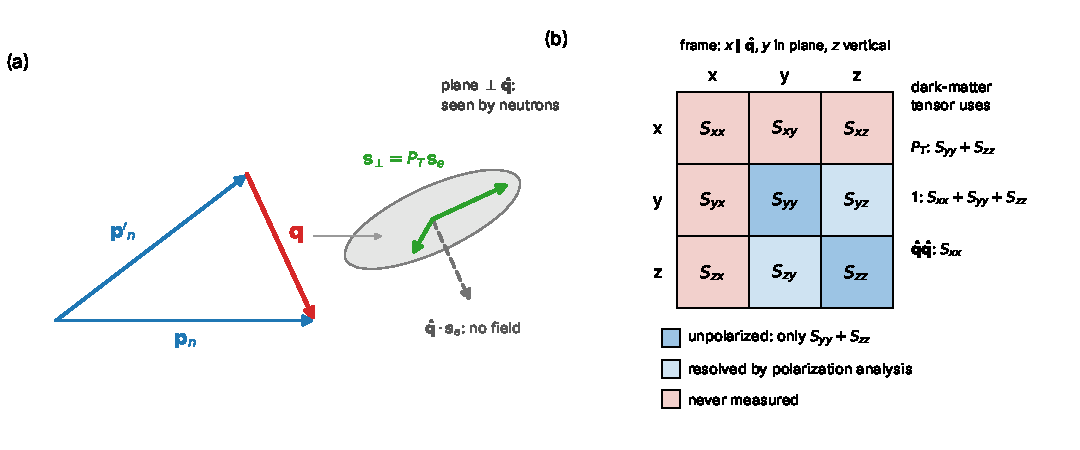
\includegraphics[width=\linewidth]{figures/ch14/fig14_4.pdf}
  \caption{The neutron geometry and the transverse projector. (a) A neutron of momentum $\mathbf{p}_n$ leaves with $\mathbf{p}'_n$ and gives the target $\vect{q} = \mathbf{p}_n - \mathbf{p}'_n$. Of the spin density at wavevector $\vect{q}$, only the part in the plane perpendicular to $\hat{\vect{q}}$, $\vect{s}_\perp = P_T\vect{s}_e$, produces a magnetic field and scatters the neutron; the component along $\hat{\vect{q}}$ produces none. (b) The spin response $S_{ab}$ in the frame with $x$ along $\hat{\vect{q}}$, $y$ in the scattering plane and $z$ vertical. Unpolarized neutrons measure the sum $S_{yy} + S_{zz}$; polarization analysis resolves the transverse block; the elements in the first row and column are not measured at this $\vect{q}$. Right-hand columns of (b): the elements that the dark-matter tensors proportional to $P_T$ (for example $\mathcal{O}_9$), to the unit matrix ($\mathcal{O}_4$) and to $\hat q_a\hat q_b$ ($\mathcal{O}_6$, $\mathcal{O}_{10}$) contract. Schematic.}
  \label{fig:14-neutron}
\end{figure}

\subsection{The longitudinal response under isotropy}\label{sec:14.4-iso}

Spin-rotation symmetry about the moments supplies the missing element at one $\vect{q}$, without a model of the spin density but with a hypothesis on the Hamiltonian: spin--orbit coupling and the dipolar interaction are neglected. In a collinear magnet with moments along $\pm\hat{\vect{m}}$, and with spin--orbit coupling neglected, the Hamiltonian is invariant under rotations of all spins about $\hat{\vect{m}}$, independently of the lattice; the Heisenberg model of \cref{sec:7.1} is the example. A rotation of the spin indices alone then leaves $S_{ab}(\vect{q},\omega)$ unchanged at every $\vect{q}$, and the only tensors with that property are built from $\delta_{ab}$, $\hat m_a\hat m_b$ and $\epsilon_{abc}\hat m_c$:
\begin{equation*}
  S_{ab}(\vect{q},\omega) = S_\parallel\,\hat m_a\hat m_b + S_\perp\,(\delta_{ab} - \hat m_a\hat m_b) + \ii S_{\mathrm{c}}\,\epsilon_{abc}\hat m_c ,
\end{equation*}
with three functions of $\vect{q}$ and $\omega$. The one-magnon response \cref{eq:14.1-Safm} has this form with $S_\parallel = 0$, and the two-magnon response \cref{eq:14.2-S2m} is all $S_\parallel$. The antisymmetric part drops out of every symmetric contraction. With $\theta_m$ the angle between $\hat{\vect{q}}$ and $\hat{\vect{m}}$,
\begin{equation}
  \Tr\bigl[P_TS\bigr] = S_\parallel\sin^2\theta_m + S_\perp(1 + \cos^2\theta_m), \qquad
  \hat{\vect{q}}\cdot S\cdot\hat{\vect{q}} = S_\parallel\cos^2\theta_m + S_\perp\sin^2\theta_m .
  \label{eq:14.4-uniax}
\end{equation}
Polarization analysis now suffices at a single $\vect{q}$. With $\hat{\vect{m}}$ in the scattering plane at an angle $\theta_m \ne 0, \frac\pi2$ to $\hat{\vect{q}}$, the vertical element is $S_{zz} = S_\perp$ and the in-plane element $S_{yy} = S_\parallel\sin^2\theta_m + S_\perp\cos^2\theta_m$, which equals $\hat{\vect{q}}\cdot S\cdot\hat{\vect{q}}$ with $\cos$ and $\sin$ exchanged and fixes $S_\parallel$. Unpolarized data give one equation for two unknowns at each $\vect{q}$, and a second measurement is needed at another angle with the same $S_\parallel$ and $S_\perp$. That is the content of the \emph{isotropy hypothesis}: in the window used, $S_\parallel$ and $S_\perp$ depend on $\vect{q}$ only through $|\vect{q}|$, or do not change when the moments are turned at fixed $\vect{q}$. The second form is the easier one to realize. A soft magnet can be turned by an applied field with $\vect{q}$ held fixed in the crystal; a YIG sphere saturates above \SI{82}{mT} (\cref{we:14-yig}). In the spin-rotation-invariant model the two settings then measure exactly the same $S_\parallel$ and $S_\perp$, and only spin--orbit coupling and the magnetic dipolar interaction break the hypothesis. The dipolar term, $\omega_M\sin^2\theta_{\vect{q}}$ in the spin-wave energy with $\omega_M = \SI{28.5}{\micro eV}$ for YIG (\cref{we:14-yig}), is negligible above about \SI{0.1}{meV}, far below the \SI{5}{meV} where the data start. Given $P_i = \Tr[P_TS]$ at two angles $\theta_1$ and $\theta_2$, with $c_i = \cos^2\theta_i$, the solution of the two equations \cref{eq:14.4-uniax} is
\begin{equation}
  S_\parallel = \frac{P_1(1 + c_2) - P_2(1 + c_1)}{2(c_2 - c_1)}, \qquad S_\perp = \frac{P_2(1 - c_1) - P_1(1 - c_2)}{2(c_2 - c_1)} ,
  \label{eq:14.4-invert}
\end{equation}
and the longitudinal element follows from \cref{eq:14.4-uniax} for any direction of $\vect{q}$ relative to $\hat{\vect{m}}$.

A paramagnet in zero field, or a sample of many randomly oriented domains, is invariant under all rotations, so $S_\parallel = S_\perp$ and $\hat{\vect{q}}\cdot S\cdot\hat{\vect{q}} = \frac12\Tr[P_TS]$~\cite[Eq.~(35)]{berlin2025determining}. In an ordered magnet the two-magnon continuum, \SI{7.3}{\percent} of the one-magnon weight in NiO (\cref{we:14-nio}), lies entirely in $S_\parallel$, and the two-angle inversion keeps it.

\begin{workedexample}{The two-angle inversion for an isotropic paramagnet}\label{we:14-paramagnet}
Take a paramagnet in zero field, so that $S_\parallel = S_\perp = S_0$ at the $(|\vect{q}|, \omega)$ of interest, and measure $\Tr[P_TS]$ with $\vect{q}$ perpendicular and then parallel to a fixed crystal axis $\hat{\vect{m}}$: $c_1 = 0$, $c_2 = 1$. Both measurements give $2S_0$, and \cref{eq:14.4-invert} reduces to $S_\parallel = P_1 - P_2/2$ and $S_\perp = P_2/2$, which returns $S_0$ for both. The hypothesis is tested by the data themselves: $P_2 - P_1 = (c_2 - c_1)(S_\perp - S_\parallel)$ vanishes.

Errors decide whether the inversion is worth doing. Give each measurement a statistical error of \SI{5}{\percent}, $0.1S_0$, independent between the two. Then $S_\perp$ carries $0.050S_0$, while $S_\parallel$ carries $(\sqrt5/2)\times0.1S_0 = 0.112S_0$, more than twice the relative error of the data. The longitudinal element needed for $\mathcal{O}_6$ along $\hat{\vect{m}}$ is $S_\parallel$ itself, with the same \SI{11}{\percent}; at $\cos^2\theta = \frac13$ it is $P_1/3 + P_2/6$, with \SI{3.7}{\percent}. The isotropy test, $P_2 - P_1 = 0 \pm 0.141S_0$, limits $|S_\perp - S_\parallel|$ to about \SI{14}{\percent} of $S_0$ at one standard deviation.

A smaller rotation gives larger errors. With $c_2 = \sin^2 30^\circ = 0.25$ instead, the denominator $2(c_2 - c_1)$ drops from 2 to 0.5, $S_\parallel = 2.5P_1 - 2P_2$ and its error grows to $0.32S_0$, \SI{32}{\percent}. The one-angle shortcut $\frac12\Tr[P_TS]$ has the \SI{5}{\percent} of the data, but it is right only if the paramagnet is in fact isotropic, which the two-angle measurement checks.
\end{workedexample}

A spin-wave model fitted to the transverse data supplies the longitudinal element as well, and its fit uncertainty enters as a normalization (\cref{sec:8.8}); a longitudinal response measured at dark-matter momenta, without such a model or the localized-moment form, does not exist.
